I decompose TOU-tariff-causing reductions in household electricity consumption around the peak rate period into two parts to determine the share of electricity savings stemming from two distinct sources: savings from non-temperature-control and temperature-control electricity uses. Here, the non-temperature-control-related electricity savings mean the reductions in electricity demand that are stably achievable regardless of each day's weather conditions, especially temperatures. That is, the savings associated with non-temperature-control electricity uses do not vary across days. On the contrary, the latter savings strictly depend on daily HDDs, which fluctuate daily. Specifically, temperature-control-associated electricity savings are additional savings that appear only on days with non-zero daily HDDs due to for-heating electricity consumption in households. Isolating the impact of the TOU prices on household electricity demand for temperature-control uses from the total reductions in electricity demand enables us to know how differently the TOU tariff structures function from day to day, whose implications will be discussed later.

To break down household responses to the TOU program around the peak rate period, I exploit the following DID-style spline regression model\footnote{Table XYZ shows point estimates that are from a nonparametric model. The U-shaped ATEs across daily HDDs substantiate the use of the DID-style spline regression model in \ref{Eq:Model-Specification_Breakdown-of-Hourly-Average-Treatment-Effect}.}:
\begin{equation}
\small
\begin{split}
    kWh_{ith} \ 
    & = \ \beta_{1} HDD_{t} \ + \ \beta_{2} HDD_{t}^{*} \\
    & \hspace{0.7cm} + \ \beta_{3} \mathds{1}[\text{Treatment}]_{i} \ + \ \beta_{4} HDD_{t} \mathds{1}[\text{Treatment}]_{i} \ + \ \beta_{5} HDD_{t}^{*} \mathds{1}[\text{Treatment}]_{i} \\
    & \hspace{0.7cm} + \ \beta_{6} \mathds{1}[\text{Post}]_{t} \ + \ \beta_{7} HDD_{t} \mathds{1}[\text{Post}]_{t} \ + \ \beta_{8} HDD_{t}^{*} \mathds{1}[\text{Post}]_{t} \\
    & \hspace{0.7cm} + \ \beta_{9} \mathds{1}[\text{Treatment \& Post}]_{it} \ + \ \beta_{10} HDD_{t} \mathds{1}[\text{Treatment \& Post}]_{it} \ + \ \beta_{11} HDD_{t}^{*} \mathds{1}[\text{Treatment \& Post}]_{it} \\
    & \hspace{0.7cm} + \ \alpha_{dw} \ + \ \epsilon_{ith}
\end{split}
\label{Eq:Model-Specification_Breakdown-of-Hourly-Average-Treatment-Effect}
\end{equation}
Like (\ref{Eq:Model-Specification_Hourly-Average-Treatment-Effects}), the dependent variable $kWh_{ith}$ is the electricity consumption by household $i$ on the day $t$ during the hour of the day $h$. There are three indicator variables in the model: the first indicator variable $\mathbb{1}[\text{Treatment}]_{i}$ has the value of 1 if household $i$ is assigned to the treatment group; the second indicator variable $\mathbb{1}[\text{Post}]_{t}$ equals 1 when the day $t$ is in the treatment period; the last indicator variable $\mathbb{1}[\text{Treatment \& Post}]_{it}$ is equal to 1 only for treatment households in the treatment period. The model also includes interaction terms between HDD-relevant terms and those indicator variables. In the econometric model, $HDD_{t}$ means the daily heating degree days on the day $t$. And $HDD_{t}^{*}$ is required to introduce nonlinearity in HDD-associated response to TOU pricing.\footnote{Mathematically, $HDD_{t}^{*}$ is defined as follows:
\begin{equation*}
    HDD_{t}^{*} \ = \ (HDD_{t} - Knot) \ \times \ \mathbb{1}[HDD_{t} > Knot],
\end{equation*}
where $Knot$ is a reference value at which the slope of the predicted line starts to change.
} The terms $\alpha_{iw}$, $\gamma_{dw}$, and $\delta_{mw}$ are household-by-half-hourly-time-window, day-of-week-by-half-hourly-time-window and month-of-year-by-half-hourly-time-window fixed effects, respectively. 

The primary coefficients of interest in (\ref{Eq:Model-Specification_Breakdown-of-Hourly-Average-Treatment-Effect}) are $\beta_{9}$, $\beta_{10}$, and $\beta_{11}$. The three coefficients show how much electricity consumption the households assigned to the treatment group reduced after deploying the TOU program compared to those in the control group. To be specific, $\beta_{9}$ demonstrates the decrease in residential electricity consumption for non-for-heating uses. Both $\beta_{10}$ and $\beta_{11}$ collectively mean the reductions in electricity consumed to satisfy household heating needs at given daily HDDs. 

\begin{figure}[!th]
\centering
%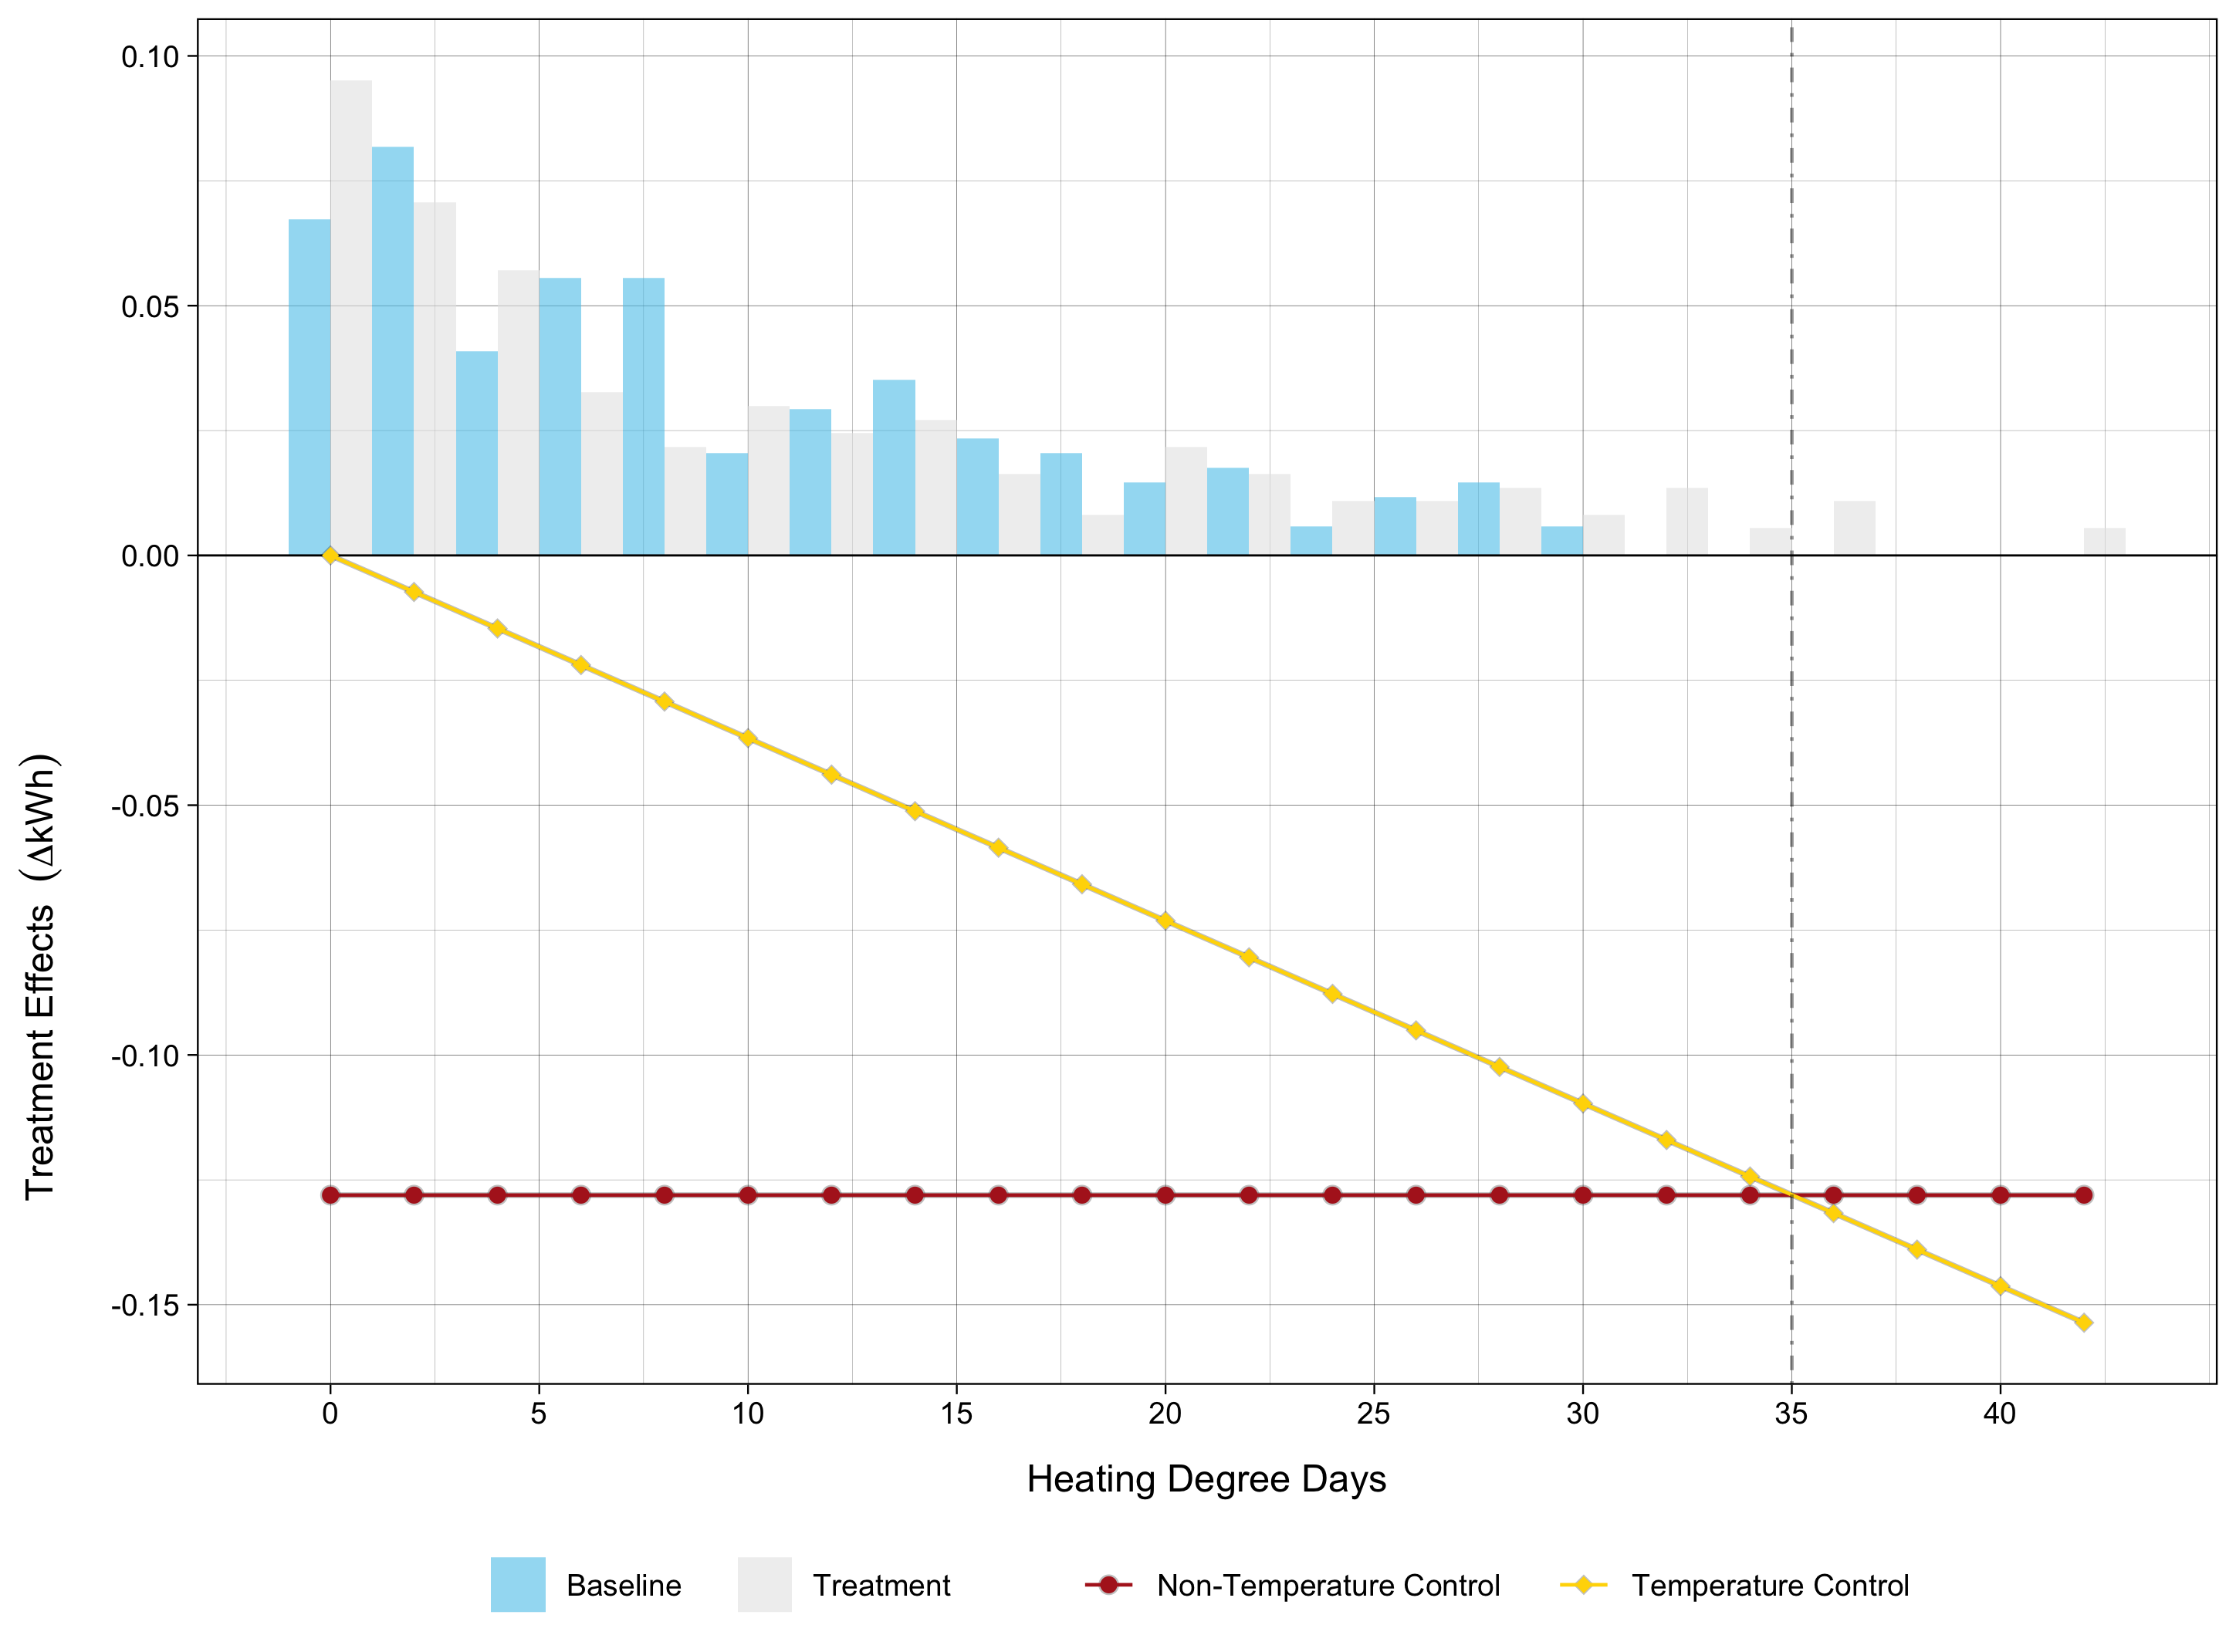
\includegraphics[scale = 0.16]{03_Chapter-2/00A_Figures/Figure_Breakdown-of-Hourly-ATEs-in-the-Peak-Rate-Period.png}
\caption{Breakdown of Hourly Average Treatment Effects}
\label{Figure:Breakdown-of-Hourly-ATEs-in-the-Peak-Rate-Period}
\end{figure}

Using the point estimates of the three coefficients of interest provided in Table \ref{Table:Breakdown-of-Average-Treatment-Effects-in-the-Peak-Rate-Period}, I graphically summarize the predicted reductions from each of the two sources of electricity savings in Figure \ref{Figure:Breakdown-of-Hourly-ATEs-in-the-Peak-Rate-Period}. Regarding the savings in electricity consumption for non-temperature-control uses, which are independent of weather conditions, the figure clearly shows that the treated households significantly reduced their consumption when they were subject to peak-hour prices. Their non-for-heating electricity consumption also decreased in both pre- and post-peak intervals, albeit relatively smaller in magnitude. The changes in temperature-control-use-associated electricity consumption occurred as well in all three intervals, but its evolving pattern over daily HDDs was quite different in each interval. Specifically, the impact of TOU pricing on residential electricity consumption for heating is U-shaped in the peak rate period, while it is salient only when daily HDDs are sufficiently large in the two off-peak intervals. In other words, from the figure, it is evident that the savings originating from for-heating-purpose household electricity consumption are a nonlinear function of daily HDDs in all three intervals.

The specification (\ref{Eq:Model-Specification_Breakdown-of-Hourly-Average-Treatment-Effect}) is also utilized to examine, during the peak rate period, the relationship between the degree of price increases and the electricity savings. The by-tariff-group estimates of the coefficients of interest are presented in Table \ref{Table:Breakdown-of-Average-Treatment-Effects-in-the-Peak-Rate-Period}. As shown in the table, on the whole, the savings from electricity demand for non-temperature-control uses tend to be proportional to the size of price risings in peak hours. Moreover, the marginally diminishing effects of TOU pricing, discussed in \cite{Peaking-Interest:How-Awareness-Drives-the-Effectiveness-of-Time-of-Use-Electricity-Pricing_Prest_2020}, seem not to be championed by my point estimates. And the two estimates associated with temperature-control-use-related electricity savings (i.e., $\hat{\beta}_{10}$ and $\hat{\beta}_{11}$) are statistically significant only for the case of the smallest price increase (i.e., only for the Tariff Group A). Jointly, those findings imply two points. First, household reaction to the TOU prices in peak hours differs in non-temperature- and temperature-control uses. Second, the savings from non-for-heating electricity consumption do not behave as expected from the previous study. Inspired by those implications, I formulate the resulting variations in household electricity consumption as a linear function of the magnitude of rate changes in the peak-demand hours in the following section.

%\begin{table}[!th]
% Add the title
\caption{Breakdown of Average Treatment Effects in the Peak Rate Period}
\label{Table:Breakdown-of-Average-Treatment-Effects-in-the-Peak-Rate-Period}
\centering
% Determine font size
\small
% The number of "c" is equal to the number of columns. And determine the width
% of each column.
\begin{adjustbox}{scale = 0.8}
\begin{tabular}{@{\extracolsep{5pt}}lccccccc}
\\[-5.5ex]
\hline \hline
\\[-3.0ex]
% Add the label of the dependent variable. And the number must be the same with
% the number of columns.
& \multicolumn{7}{c}{Hourly Electricity Consumption  (kWh/Hour)} \\
\\[-3.0ex]
% The range must be "2-(The number of columns + 1)"
\cline{2-8}
\\[-3.0ex]
%& All & All & All & Tariff A & Tariff B & Tariff C & Tariff D \\
%\\[-4.0ex]
& (1) & (2) & (3) & (4) & (5) & (6) & (7) \\
\\[-3.0ex]
\hline
\\[-2.0ex]
HDDs & 0.005$^{**}$ & 0.005$^{**}$ & 0.004$^{**}$ & 0.004$^{*}$ & 0.006$^{***}$ & 0.006$^{**}$ & 0.007$^{***}$ \\
& (0.002) & (0.002) & (0.002)  & (0.002) & (0.002) & (0.002) & (0.002) \\
& & & & & & & \\
$\mathbb{1}$[Treatment] & 0.077$^{***}$ & & \\
& (0.030) &  & \\
& & & & & & & \\
$\mathbb{1}$[Treatment] $\times$ HDDs & 0.003$^{**}$ & 0.003$^{**}$ & 0.004$^{**}$ & 0.005$^{***}$ & 0.004 & 0.002 & 0.001 \\
& (0.001) & (0.002) & (0.002) & (0.002) & (0.003) & (0.002) & (0.002) \\
& & & & & & & \\
$\mathbb{1}$[Post] & 0.001 & 0.001 & & 0.00002 & 0.002 & 0.001 & 0.001 \\
& (0.018) & (0.019) & & (0.019) & (0.019) & (0.019) & (0.019) \\
& & & & & & & \\
$\mathbb{1}$[Post] $\times$ HDDs & $-$0.001 & $-$0.001 & & $-$0.0005 & $-$0.001 & $-$0.001 & $-$0.001 \\
& (0.002) & (0.002) & & (0.002) & (0.002) & (0.002) & (0.002) \\
& & & & & & & \\
$\mathbb{1}$[Treatment \& Post] & $-$0.128$^{***}$ & $-$0.128$^{***}$ & $-$0.127$^{***}$ & $-$0.099$^{***}$ & $-$0.122$^{***}$ & $-$0.138$^{***}$ & $-$0.182$^{***}$ \\
& (0.015) & (0.016) & (0.015) & (0.019) & (0.026) & (0.019) & (0.025) \\
& & & & & & & \\
$\mathbb{1}$[Treatment \& Post] $\times$ HDDs & $-$0.004$^{***}$ & $-$0.004$^{***}$ & $-$0.004$^{***}$ & $-$0.004$^{***}$ & $-$0.005$^{***}$ & $-$0.003$^{*}$ & $-$0.003 \\
& (0.001) & (0.001) & (0.001) & (0.001) & (0.002) & (0.001) & (0.002) \\
& & & & & & & \\
\hline
\\[-2.0ex]
Tariff Group & All & All & All & A & B & C & D \\
FEs: ID by Half-Hourly Time Window & No & Yes & Yes & Yes & Yes & Yes & Yes \\
FEs: Day of Week by Half-Hourly Time Window & Yes & Yes & Yes & Yes & Yes & Yes & Yes \\
FEs: Month of Year by Half-Hourly Time Window & Yes & Yes & Yes & Yes & Yes & Yes & Yes \\
Observations & 3,522,560 & 3,522,560 & 3,522,560 & 1,771,600 & 1,147,240 & 1,795,680 & 1,155,840 \\
Adjusted R$^{2}$ & 0.051 & 0.366 & 0.366 & 0.361 & 0.377 & 0.362 & 0.360 \\
\\[-2.0ex]
\hline \hline
\\[-4.5ex]
\end{tabular}
\end{adjustbox}
\begin{tablenotes}
    \footnotesize
    \textit{Note}: (...)  % Add a note.
\end{tablenotes}
\label{Table:}  % Add the label
\end{table}

